
\chapter{Réflexions}


Y-a-t-il une modification de l'écoute du patient lors de séances en musicothérapie?
Est-ce visible et lisible au moyen du test d'écoute employé?
Peut-on définir et retracer un chemin sonore psychologique du patient au moyen d'un test d'écoute?


Selon les hypothèses évoquées, nous avons été amenés aux réflexions suivantes.

Nous utilisons un outil qui est le son. Nous accompagnons
le patient d'un point A pour aller au point B : que s'est -il passé
dans son écoute?
En comparant les données, nous pouvons observer des résultats visibles et tangibles 
d'une transformation de la
perception basée sur un test de reconnaissance de sons;  qui permet de visualiser une transformation psychologique
de l'écoute. 


Il y a des résultats : nous pouvons faire un constat.
Ce sont des données pouvant servir à mieux comprendre le patient
et à l'accompagner dans son cheminement thérapeutique.


\subsection{L'anamnèse et le bilan en musicothérapie}

  Avant d'amorcer une thérapie, le test effectué fournit des renseignements, toujours basés sur le son, qui seront complémentaires à l'anamnèse. Nous pouvons donc l'inclure dans un  bilan en musicothérapie.

  \
\subsubsection{La communication}


  
\begin{itemize}
  \item Les questions/réponses inhérents au 
 test d'écoute provoque le dialogue. Le patient est amené de façon
 détournée à se livrer et à évoquer des détails auxquels il
 n'aurait pas prêté attention. L'anamnèse prend donc ici un autre
 caractère puisqu'elle est complétée par le son et l'écoute.

	 La relation avec le patient est indispensable à créer pour toutes thérapies. Le test peut créer dès le premier entretien une alliance thérapeutique.
	Le test représente une procédure claire qui peut être
        considéré comme un outil utile pour instaurer un dialogue avec
        le patient et servir d' indication sur le plan du travail à
        envisager.
  \end{itemize}      
\paragraph{Le test d'écoute est une forme d'intervention
  musicothérapeutique}

Le test d'écoute est en soi une forme d'intervention
 musicothérapeutique puisqu'il 
 a deux rôles intrinsèques:

 la création d' une alliance thérapeutique et
     travail avec le son avec l'implication directe du
     patient dans le rôle de la 
     reconnaissance de sons
         Il comporte un travail immédiat avec le son en impliquant le patient
 dans le rôle actif de leur reconnaissance. Il fait faire un travail de reconnaissance de sons dans
 l'espace (repérage de fréquences selon le volume). Le patient
 participe activement en fixant son attention sur les
 sons émis par l'appareil et transmis aux écouteurs en les repérant
  puis en y
 répondant. Cette implication directe conduit le patient à créer par lui-même et de manière
 inconsciente  
 son propre espace; ce  qui permettra par là même déjà d'entamer, pour certains dumoins, leur propre
 processus thérapeutique. (40% participe à la réussite d'une
                             % thérapie,(Sandra Lutz Hochreutener)
 Il peut être perçu comme un cadre médical  rassurant par nombre de patients, jouant son rôle de soutien dans la prise en charge.
  
 
En cours de la thérapie, il peut être utile d'évaluer, tout
comme se servir lors d'un voyage d'une jauge pour estimer le chemin parcouru et celui
qui reste à faire, en cas d'interrogations, de doutes dans la façon de procéder.
En fin de thérapie, il permet d'évaluer la transformation.


\paragraph{La visibilité}

Deux aspects ressortent distinctement: la visibilité et la visualisation.

La visibilité: être visible par le son est une façon de se concrétiser extérieurement en en prenant conscience: une forme de ``comportementalisme de l'audition'' .


La visualisation: se visualiser par son chemin d'écoute.  
Ce processus de visualisation tente de matérialiser l'abstraction innée dues aux propriétés du son, l'aspect intemporel et éphémère du son entre l'écoute et la vue.
Il permet de se situer dans l'espace sonore et, en un même temps, induit une prise de conscience et de distance avec soi-même. Tout le corps, physique et psychique est impliqué (--- tendre l'oreille---) avec toutes les fonctions cognitivo-proprioceptives.


Le patient obtempère aux consignes du thérapeute, fait un choix parmi des sons précis, dialogue sur les résultats, tout ceci relève déjà d'une volonté de changement intérieur, en  éveille tout au moins cette idée de déclenchement d'un travail, initie un début de cheminement intérieur.
Être accompagné dans la lecture de son évolution sonore permet de constater un résultat qui  peut le conforter ou non dans son sentiment intérieur.
	
	D'autre part, le rôle du patient est différent dans son essence même, non pas dans le sens de "patere" souffrir et subir, mais valorisé dans celui du rôle actif qu'il peut jouer : celui-ci peut se rendre compte de sa capacité à influencer sa façon d'écouter, qu'il a une présence signifiante dans sa thérapie.  Il n'est pas passif. Bien sûr, cela peut paraître une évidence car on sait l'impact de la musique sur le corps tout entier. Mais ici on rejoint  le concept de musique intégrative déjà cité\autocite[Cf.]{vrait_musicotherapie_2018}. Le patient peut être nourri par la musique mais n'est pas "passif" et seulement l'"objet " qui bénéficie du traitement musical. Son  écoute lui appartient en propre, elle est personnelle et modifiable. S'il y a modification, il peut y avoir un changement; et le mot "changement" prend alors une connotation différente,  le mouvement est y  sous-entendu,  une démarche peut en découler, voire une évolution. 


  \section{Les instruments et leur fréquence }
 De manière très pragmatique, le test peut être
considéré comme un indicateur des zones de fréquences à
privilégier dans le travail avec le patient. Chaque instrument a une tessiture
différente avec une plage
définie de fréquence. Selon l'analyse de l'écoute du patient, le choix
d'instrument à privilégier sera plus rapide et plus sûre.

      \begin{figure}
	\centering
	\includegraphics[width=1\linewidth]{images/instrumentfréq.pdf}
	\caption[Les instruments et leurs fréquences]{Ilustration des instruments avec leurs fréquences}
       
	\label{instrumentfreq}
\end{figure}
  



\section{Graphique: Zones 1-2-3 du Test d'écoute // Musicothérapie}


        \begin{figure}
	\centering
	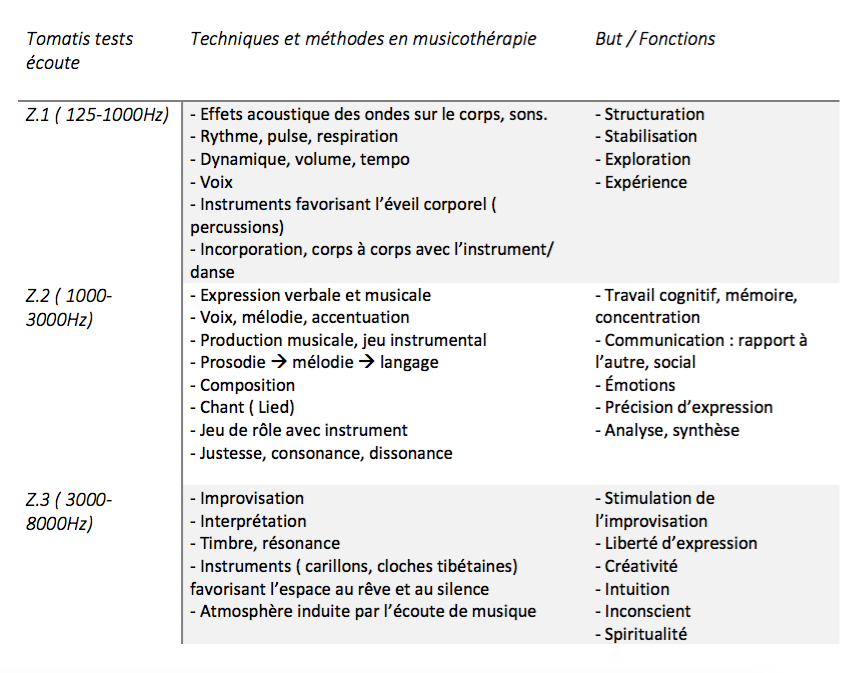
\includegraphics[width=1\linewidth]{images/testtechnmethbut}
	\caption[Zones du test avec la musicothérapie]{Schéma des
          zones avec leur application en musicothérapie}
       
	\label{testbutetfonction}
\end{figure}



S'il n'y a pas de changement visible dans le test, quelles conclusions
peut-on en tirer ? le changement va-t-il toujours de pair avec le
patient? synchronisé ou différencié dans le temps?
Comme pour toutes thérapies, le patient doit avoir le temps de l'intégrer. Quand
il aura été amené à une certaine prise de distance par rapport à
lui-même et à son environnement, il passera par différentes phases qui peuvent être celles de l'acceptation, que ce soit celle de son identité, de sa transformation, ou d'un changement dans ses habitudes --- de quitter le confort de ceux-ci même si elles sont jugées négatives par lui-même et par les autres --- . Tout ceci prend du temps et ne peut pas 
toujours  aller en simultanéité avec des résultats immédiats, avant/ après.

\subsection{Critiques: }

Par cette démarche, il y a le risque de catégoriser le patient. Les
rapports doivent rester confidentiels et en aucun cas transmis
aux assurances-maladies.
Du côté du patient, s'il est toujours en
attente de résultats, cette façon de faire peut le figer dans son parcours  Ou, au contraire, ce peut être une aide 
dans son travail, son évolution. Ces deux possibilités sont
intrinsèques à tous les tests.

Les séances de musicothérapie se sont déroulées mais  n'ont pas été
décortiquées et analysées. Ce serait passionnant de le faire mais ce n'était pas l'objectif de ce travail.		
        
 

Différents paramètres inhérents à ce type d'étude sont à
considérer. Que ce soit le manque de temps, les départs imprévus des patients, et/ou leur
absence momentanée (visite du psychologue, maladie, etc.). rajoutés à la
contingence difficile due à la distance séparant le lieu de domicile à
celui du lieu d'étude, toutes ces contingences ont été les principaux facteurs réducteurs de
tests valables.
: comment planifier un départ imprévu d'un patient !? il a fallu parfois
faire beaucoup de route pour effectuer les tests finaux d'un ou deux
patients.
  
Par conséquent,  de nombreux tests sont restés 
incomplets et n'ont pu
être validés car ils ne remplissaient pas toutes les conditions requises.  En définitive, sur 40 tests d'écoute Tomatis et 26 tests
WHOQO-Bref, nous avons choisi de ressortir l'étude pour le groupe A de
5 patients effectifs en musicothérapie, tests complets, et le groupe
témoin B de 5 patients sur 9 effectifs, sans musicothérapie et tests
complets. 
 
De manière très générale, les résultats obtenus ne
  sont pas significatifs.  La prise en charge en musicothérapie a eu lieu
  une fois par semaine pendant une heure, ce qui semble trop court pour observer un changement important. Nous pourrions émettre la supposition suivante :  est-ce qu'un un travail journalier, régulier aurait été indiqué pour des résultats plus rapidement visibles avec le test?
  Est-ce qu'une immersion plus intensive en musicothérapie transformerait l'écoute des patients ? 
   En comparaison avec des
  modifications importantes de courbes des tests observées généralement  lors d' une écoute
  régulière de deux heures par jour de musique pendant 15 jours --- en référence à l'entrainement des muscles de l'oreille chez Tomatis, qui, nous le rappelons, est une pédagogie de l'écoute --- il aurait été intéressant de pouvoir faire cette étude comparative dans cette clinique. Ainsi, nous aurions pu éventuellement mettre en avant  l'absolue nécessité de créer et d'instaurer systématiquement la musicothérapie dans de nombreuses institutions mais aussi  de la développer beaucoup plus intensément  si elle est déjà existante.
  Nous sommes clairement en présence d'une ébauche d'études, avec des pistes
  suggérées. 
  Cette étude est un mixe: quantitatif et qualitatif. Nous avons ainsi pris l'option de nous tenir à une
  observation, celle de la transformation de l'écoute.
  
 \paragraph{Un cas particulier qui mérite réflexion:}

 A fortiori, relevons le cas fort intéressant  d'une patiente du groupe B (sans
  musicothérapie) : lors du test, surprise d'abord d'apprendre, en visualisant son
  écoute, que la musique pouvait la modifier, cette patiente s'est
  mise à écouter assidûment de la musique de Mozart pendant son séjour en clinique, entre le 1° test et le second test.  Les résultats
  graphiques obtenus lors de sa sortie sont clairement significatifs
  et de plus sont en concordance avec le WHOQ-Bref!  
  Par conséquent, le test d'écoute a permis de lui faire prendre conscience d'une part que son écoute lui appartenait personnellement et d'autre part, qu'elle pouvait elle-même avoir un impact et jouer un rôle non seulement sur son écoute mais aussi sur sa propre  transformation.
Il est clair, selon Sandra Lutz Hochneutener, que la réussite d'une
thérapie réside à 40%  chez le patient.


  

\begin{itemize}
\item Est-ce que ce test pourrait être un outil pour les thérapeutes et
les patients ? 
\item Avoir un support réel, visible car graphique pourrait-il être d'une
quelconque utilité pour le thérapeute ?
\item Est-il possible, à partir de deux tests d'écoute, de tirer des hypothèses
sur l'impact du son, de la musicothérapie, du soin par le son, sur
un patient ?
\item Le patient reste au centre de nos préoccupations.
\item Serait-ce une façon de démontrer l'utilité de la musicothérapie
pour une plus large acceptation de 
cette thérapie dans plus de milieux hospitaliers ou autres ?


\end{itemize}

\section{La musicothérapie et la méthode Tomatis}

La musicothérapie et la méthode Tomatis sont des concepts très différents. Bien que la notion d'écoute les réunit, bien que leur medium soit la musique et plus particulièrement le son, d'un côté il s'agit d'une thérapie et de l'autre, il s'agit d'une pédagogie, d'un entrainement de la musculature de l'oreille. 
Tomatis se focalise et opère essentiellement sur le capteur auditif (vestibulo-cochléaire) pour amener, par ce processus, le patient à une certaine  amélioration par rapport à sa vie actuelle, à des souhaits ou à des attentes précises; celle-ci peut se réaliser au niveau du langage et ce, par l'intermédiaire de la musique et du chant. Nous pouvons de notre côté  émettre l'hypothèse que si le contrôle auditif est de bonne qualité ainsi que l'émission vocale, c'est-à-dire que la boucle phono-auditive est élaborée sans problème, l'oreille est prête, même peut-être plus prête et apte à travailler beaucoup plus en profondeur avec tous les riches moyens que la musicothérapie propose.
Préparer le terrain, faire un travail physique de fond, une
préparation de l'oreille pour que celle-ci soit totalement
opérationnelle et prête à aborder si nécessaire, un travail en
musicothérapie sur le plan physique ou psychique. simplement pour se
sentir bien sa peau, bien dans son âme.
Voilà l'hypothèse énoncée et ce que nous nous pouvons conclure, en effet.


        Est-ce utile à tout musicothérapeute d'avoir un appareil test d'écoute ? certainement pas. C'était un moyen de faire cette étude.
     Nous nous sommes  limités ici intentionnellement
     à ce concept de test.
 La matière sonore est la matière première de la  musicothérapie. 
 Par son biais, elle  apporte de multiples éléments d'évaluation du
 sujet. 
 Certains  intégrent plus que d'autres dans leur pratique des techniques relevant du domaine de la psychothérapie--de l' analytique, 
  du comportementalisme, du cognitivisme, de la  systémique ainsi que
  celles dites humanistes.  Le concept de "médium malléable" a été
  développé par  R.Rousillon\footnote{R.Rousillon,\textit{Paradoxes et situations limites,  
  		de la psychanalyse} Paris, Puf. 1991} 
  et qu'il est possible de transposer dans la matière \textit{musique} 
  pour "favoriser et accompagner le processus 
  de symbolisation"\footnote{F.X.Vrait, \textit{La musicothérapie},Ch.3, p. 112}.

 Le musicothérapeute est un être extrêment sensible avec de multiples
 ``antennes'' : l'intuition reste primordiale tout autant que  
 l'écoute. L'oreille se dresse pour une écoute empathique, pour ``rester en contact émotionnel  
 avec le patient'' , Eckert (2007) par le son qui va au plus profond de
 l'être.

 
\begin{quotation}
	\char`\"{}\textbf{``L'oreille est l'organe le plus sensible des sens 
et l'instrument de diagnostic  le plus important du
musicothérapeute.'' `\"{``Hören Musiktherapeuten anders?'' }Thomas
Stegemann, Vienne/ Seminar Zürich ZHdK, 2017.}
 	
\end{quotation}
La musicothérapie fait partie de ces thérapies dites subtiles. Elle
est très difficilement quantifiable. La
psychologie cognitivo-comportementaliste peut le quantifier avec des tests et semble avoir gagné depuis en crédibilité. Mais avec la musicothérapie ou d'autres formes de thérapie, il n'y a
jamais, à proprement parlé, d'avant et d'après mais il y a transformation.
Et les transformations échappent toujours aux quantifications. Peut-être
ici pourrons-nous apporter un outil plus objectif par un test particulier
d'écoute : la démonstration d'un travail d'écoute, d'une perception
différente, d'une sensibilité nouvelle du patient. 


% OGA: source citation Malraux

\paragraph{Apprendre à écouter}

Apprendre à écouter,
c'est un travail et des résultats pourraient être visibles.
Comme l'exprime à juste titre André Malraux : \enquote{\emph{Le monde de
	l'art n'est pas celui de l'immortalité, c'est celui de la métamorphose.}}
De même, la musique est un art produit par l'homme et qui a un impact
sur lui-même. Les deux interagissent, s'interpénètrent et s'auto-transforment
au cours des siècles.
 Ce que nous pouvons constater lors de l'aboutissement
d'une thérapie n'est pas de trouver une autre personne mais une transformation
de la perception de celle-ci par rapport au monde qui l'entoure. 
Selon
ce que nous vivons, nous nous transformons et continuons à être
soi. Nous ``sommes soi" mais autrement. Nous ne perdons
pas notre identité.


\paragraph{La musique vient dans la chair}


“La musique vient dans la chair comme un produit immatériel
qui vient travailler la zone à soigner. (...)

Je pompe de la
guérison. (...)

Depuis le début des écoutes, j’ai la sensation physique et
psychique de la
transformation. (...)

La musique est équilibrante et guérisseuse, ma zone
anesthésiée se remet à vivre, elle est remise en activité. (...)

Il y
a comme un consentement cellulaire. (...)
La béance s’estompe, cette
partie redevient comme les autres.


Apaisement. Consentement. Réconciliation.”
                                     (Une patiente, V.)